%% LyX 2.0.1 created this file.  For more info, see http://www.lyx.org/.
%% Do not edit unless you really know what you are doing.
\documentclass[english,aps,manuscript]{revtex4}
\usepackage[T1]{fontenc}
\usepackage[latin9]{inputenc}
\setcounter{secnumdepth}{3}
\usepackage{verbatim}
\usepackage{textcomp}
\usepackage{amsmath}
\usepackage{amssymb}
\usepackage{graphicx}
\usepackage{esint}

\makeatletter
%%%%%%%%%%%%%%%%%%%%%%%%%%%%%% Textclass specific LaTeX commands.
\@ifundefined{textcolor}{}
{%
 \definecolor{BLACK}{gray}{0}
 \definecolor{WHITE}{gray}{1}
 \definecolor{RED}{rgb}{1,0,0}
 \definecolor{GREEN}{rgb}{0,1,0}
 \definecolor{BLUE}{rgb}{0,0,1}
 \definecolor{CYAN}{cmyk}{1,0,0,0}
 \definecolor{MAGENTA}{cmyk}{0,1,0,0}
 \definecolor{YELLOW}{cmyk}{0,0,1,0}
}

%%%%%%%%%%%%%%%%%%%%%%%%%%%%%% User specified LaTeX commands.
\usepackage{caption}

\@ifundefined{showcaptionsetup}{}{%
 \PassOptionsToPackage{caption=false}{subfig}}
\usepackage{subfig}
\makeatother

\usepackage{babel}
\begin{document}

\title{Free expansion of Bose-Einstein Condensates with a Multi-charged
Vortex}


\author{R.P. Teles, F.E.A. dos Santos, M.A. Caracanhas and V.S. Bagnato}


\affiliation{Instituto de F�sica de S�o Carlos, USP, Caixa Postal 369, 13560-970
S�o Carlos, S�o Paulo, Brazil}
\begin{abstract}
We based on variational method to derive analytical expressions to
describe the free expansion of a multi-charged condensate with a central
vortex. The evolution of the vortex core size and the asymptotic velocity
during free expansion was studied with the cloud released from different
harmonic trap configurations. We found that an oblate condensate shape
magnifying the effects of the vorticity in the expansion of the cloud.
Besides that, the asymptotic velocity field of the cloud dimensions
gave direct information about the interaction and circulation , being
also an important parameter to track.
\end{abstract}
\maketitle

\section{Introduction}

The remarkable discovery in BEC's physics was the nucleation of vortices
inside the Bose-Einstein condensate of Alkali atoms, with many experimental
evidence\cite{3v,rev3,turb,pethick,davis}. These vortices have quantized
angular momentum by number of particles, and they are nucleation when
the system gains a rotation, i.e., angular momentum. If the rotation
of system overcomes a critical velocity of rotation, $\Omega_{c}$,
it triggers the emergence of quantized vortices\cite{critical1,vf1,vor2,pd}.
Thus the dynamics of vortex formation, the stability dynamics and
the free expansion dynamics are the subject of several studies\cite{d1v,vi1,vi2}.
The vortex dynamics have proved of paramount importance for the understanding
of the quantum turbulence\cite{turb,liv3}, and the free expansion
is the main experimental method of measurement\cite{vp,vor1,rev3,obv,MIT}.
There are many theoretical works about vortex latices and vortex in
rotating traps \cite{aa,fad,obv,pethick,rev2,dsv}, where the starting
point is the Gross-Pitaeviskii equation (GPE) \cite{gpe1,gpe2}.

In this paper we considered a muli-charged vortex at the center of
the condensate, which is the center of the harmonic trap. Here, we
used the variational method to study the effects that arise while
the free expansion of condensate, as consequence of non-fundamental
vortices. A similar works was done by E. Lundh \emph{et al}\cite{emil}
to the case where the vortex has only one quantum of circulation,
which the same work can be found with quite numeric character in Micheli
\emph{et al}\cite{michele}.

The section II present the theoretical methods used in this work.
In the section III, we have search for a suitable trial function and
analyses this one to determine the radii of condensate. Soon after
it, in the sections IV and V, we found the initials condition and
the motion equations to the free expansion, and also take the TF-limit
to the both.

Finally, the section VI has the discussions and outlooks about our
results by the method employed.




\section{Theoretical Method}

At absolute zero temperature in the absense of thermal cloud the system
is exactly described by GPE:
\begin{equation}
i\hbar\frac{\partial\Psi(\vec{r},t)}{\partial t}=\left[-\frac{\hbar^{2}}{2m}\nabla^{2}+V(\vec{r})+U_{0}\left|\Psi(\vec{r},t)\right|^{2}\right]\Psi(\vec{r},t).\label{eq:1.1}
\end{equation}
The harmonic trap is described in cylindrical coordinates as $V(\vec{r})=\frac{1}{2}m\omega_{\rho}^{2}(\rho^{2}+\lambda^{2}z^{2})$,
where $\lambda$ is the anisotropic parameter, and the constant of
mean-field interaction is $U_{0}=4\pi\hbar^{2}a_{s}/m$. Following
the variational principle we can write the Lagrangian density $\mathcal{L}$
which recoves the GPE for a complex field $\Psi(\vec{r},t)$, thus
$\mathcal{L}$ is writed as
\begin{equation}
\begin{array}{c}
\mathcal{L}={\displaystyle \frac{i\hbar}{2}\left(\Psi^{*}(\vec{r},t)\frac{\partial\Psi(\vec{r},t)}{\partial t}-\Psi(\vec{r},t)\frac{\partial\Psi^{*}(\vec{r},t)}{\partial t}\right)}\\
\\
{\displaystyle -\frac{\hbar^{2}}{2m}\left|\nabla\Psi(\vec{r},t)\right|^{2}-V(\vec{r})\left|\Psi(\vec{r},t)\right|^{2}-\frac{U_{0}}{2}\left|\Psi(\vec{r},t)\right|^{4}}.
\end{array}\label{eq:1.2}
\end{equation}
Where $\Psi(\vec{r},t)$ can be aprproximated by a trial function
$\Psi_{\ell}(\vec{r},t)$ which depends on a set of variational parameters
$q_{i}=q_{i}(t)$\cite{perez1,perez2}. This function can them be
substituted into

\begin{equation}
L=\int\mathcal{L}d^{3}r,\label{eq:1.3}
\end{equation}
in such a way that their time evolution is given by

\begin{equation}
\frac{\partial}{\partial t}\left(\frac{\partial L}{\partial\dot{q}}\right)-\frac{\partial L}{\partial q}=0.\label{eq:1.4}
\end{equation}


In that way, the next step is to find a suitable trial function.


\section{Finding a trial function}

In the central vortex case with multiplied charge, the wave functions,
in cylindrical coordinates, is given by: 
\begin{equation}
\psi_{\ell}(\rho,\phi,z)=f_{\ell}(\rho,z)e^{i\ell\phi},\label{eq:2.1}
\end{equation}
where $f_{\ell}(\rho,z)$ is the amplitude of the wave function, and
$e^{i\ell\phi}$ is a phase which carries the information of the velocity
field, where $\ell$ is integer and means the quantum number of circulation.
Therefore, by introducing \ref{eq:2.1} in time-independent GPE we
have a centrifugal term, which comes from phase $e^{i\ell\phi}$.
This term is write as $\left(\frac{\hbar^{2}\ell\text{\texttwosuperior}}{2m\rho^{r}}\right)f$.
To find a suitable ansatz for multi-charged vortex, we considered
the interval of $\rho\ll\xi$, and we have neglected potential terms
from GPE. By considering only kinetic terms with the additional centrifugal
term, we need to solve
\begin{equation}
-\frac{\hbar^{2}}{2m}\left[\frac{1}{\rho}\frac{\partial}{\partial\rho}\left(\rho\frac{\partial f}{\partial\rho}\right)\right]+\frac{\hbar^{2}\ell^{2}}{2m\rho^{2}}f=0,\label{eq:2.2}
\end{equation}
this equation give us the solution for $f(\rho)$ when this is smaller
than cloud, which means the vortex solution. For $\rho>\xi$, we considered
the solution of GPE without interaction potential, the ideal gas solution,
thus our amplitude $f(\rho,z)$ is
\begin{equation}
f_{\ell}(\rho,z)=\left[\frac{N}{\pi^{\frac{3}{2}}\ell!R_{\rho}^{2\ell+2}R_{z}}\right]^{\frac{1}{2}}\rho^{\ell}\exp\left(-\frac{\rho^{2}}{2R_{\rho}^{2}}\right)\exp\left(-\frac{z^{2}}{2R_{z}^{2}}\right),\label{eq:2.3}
\end{equation}
and now, the trial function is given by:
\begin{equation}
\Psi_{\ell}(\rho,\phi,z,t)=\psi_{\ell}(\rho,\phi,z)\exp\left(iB_{\rho}\frac{\rho^{2}}{2}\right)\exp\left(iB_{z}\frac{z^{2}}{2}\right).\label{eq:2.4}
\end{equation}
Where the parameters $R_{\rho}$, $R_{z}$, $B_{\rho}$ and $B_{z}$
are time-dependent.

If $\ell=0$, we recover the solution for a condensate without vortex
of V.M. P�rez-Garc�a \emph{et al}\cite{perez1}. Thus, the ansatz
describe since a fundamental condensate until condensates with multi-charged
vortex at the center of the atomic cloud. Note this: the parameters
$B_{\rho}$ and $B_{z}$ are responsible for the function curvature,
in other words, it is from these parameters that will appears the
acceleration in motion equation by the variational method. We must
take care with parameters $R_{\rho}$ and $R_{z}$, because they are
not the radii of our condensate for every values of $\ell$. In the
case, where $\ell$ is zero, $R_{\rho}$ and $R_{z}$ are the radii
in fact, but when we have $\ell>0$, the parameter $R_{\rho}$ is
the width of Gaussian at least a scale factor, and the peak of that
is in the point $R_{\rho}\sqrt{\ell}$. It\textasciiacute{}s occurs
due the absence of a parameter which separate these two information,
radius of vortex core and radius of the condensate. Thereby, absence
of these two parameters, we have all of information about vortex core
and cloud radius in the only one parameter, $R_{\rho}$. For that
reason, we will define the radius as:
\begin{equation}
\begin{array}{c}
R_{\bot}^{(\ell)}(t)=\sqrt{\left\langle \rho^{2}\right\rangle }=R_{\rho}^{(\ell)}(t)\sqrt{\ell+1}\\
\\
R_{||}^{(\ell)}(t)=R_{z}^{(\ell)}(t).
\end{array}\label{eq:2.5}
\end{equation}
The $\ell$, above of $R$, is the index about what case we are referring,
i.e., what kind of condensate within circulation. And the vortex core,
$\xi$, may be defined as: the healing length of a condensate without
vortex calculated at center of density, i.e.,
\begin{equation}
\xi^{(\ell)}=\ell\hbar\pi^{\frac{3}{4}}R_{\rho}^{(\ell)}\sqrt{\frac{R_{z}^{(\ell)}}{2mNU_{0}}},\label{eq:2.6}
\end{equation}
using the parameters, $R_{\rho}$ and $R_{z}$, of them respective
number of circulation.

Now we substited \eqref{eq:2.4}in \eqref{eq:1.2} and integrate its
ovar all space therefore the Lagrangian is
\begin{equation}
L=N\hbar\omega_{\rho}\left\{ \frac{\left(\ell+1\right)}{2}\left[\frac{1}{r_{\rho}^{2}}+\left(\dot{\beta}_{\rho}+\beta_{\rho}^{2}+1\right)r_{\rho}^{2}\right]+\frac{1}{4}\left[\frac{1}{r_{z}^{2}}+\left(\dot{\beta}_{z}+\beta_{z}^{2}+\lambda^{2}\right)r_{z}^{2}\right]+\frac{\gamma(2\ell)!}{2^{2\ell}\sqrt{2\pi}\left(\ell!\right)^{2}r_{\rho}^{2}r_{z}}\right\} ,\label{eq:2.8}
\end{equation}
where varational parameters were scaled as $R_{\rho}(t)=a_{osc}r_{\rho}(t)$,
$R_{z}(t)=a_{osc}r_{z}(t)$, $B_{\rho}(t)=a_{osc}^{-2}\beta_{\rho}(t)$
and $B_{z}(t)=a_{osc}^{-2}\beta_{z}(t)$, with the harmonic oscilator
length being $a_{osc}=\sqrt{\hbar/m\omega_{\rho}}$. And the intecation
parameter becomes dimensionless being write as $\gamma=Na_{s}/a_{osc}$.
The equation of motion are extracted from \eqref{eq:2.8} using \eqref{eq:1.4}
thus these are given by:
\begin{equation}
\begin{array}{c}
{\displaystyle \left(\dot{\beta}_{\rho}+\beta_{\rho}^{2}+1\right)r_{\rho}=\frac{1}{r_{\rho}^{3}}+\frac{\gamma(2\ell)!}{2^{2\ell-1}\sqrt{2\pi}\left(\ell+1\right)!\ell!r_{\rho}^{3}r_{z}}}\\
\\
{\displaystyle \beta_{\rho}=\frac{\dot{r_{\rho}}}{r_{\rho}}}\\
\\
{\displaystyle \left(\dot{\beta}_{z}+\beta_{z}^{2}+\lambda^{2}\right)r_{z}=\frac{1}{r_{z}^{3}}+\frac{\gamma(2\ell)!}{2^{2\ell-1}\sqrt{2\pi}\left(\ell!\right)^{2}r_{\rho}^{2}r_{z}^{2}}}\\
\\
{\displaystyle \beta_{z}=\frac{\dot{r_{z}}}{r_{z}}}.
\end{array}\label{eq:2.9}
\end{equation}


These four equations can be reduced to only two, which are:
\begin{equation}
\begin{array}{c}
{\displaystyle \ddot{r_{\rho}}+r_{\rho}=\frac{1}{r_{\rho}^{3}}+\frac{\gamma(2\ell)!}{2^{2\ell-1}\sqrt{2\pi}\left(\ell+1\right)!\ell!r_{\rho}^{3}r_{z}}}\\
\\
{\displaystyle \ddot{r_{z}}+\lambda^{2}r_{z}=\frac{1}{r_{z}^{3}}+\frac{\gamma(2\ell)!}{2^{2\ell-1}\sqrt{2\pi}\left(\ell!\right)^{2}r_{\rho}^{2}r_{z}^{2}}}.
\end{array}\label{eq:2.10}
\end{equation}



\section{Stationary case}

By calculate the functional energy using \eqref{eq:2.1} we obtain
each contribution which the circulation carries. Thus, the energy
of condensate with $\ell$ quanta of circulation is: 
\begin{equation}
E_{\ell}=N\hbar\omega_{\rho}\left[\frac{\left(\ell+1\right)}{2}\left(\frac{1}{r_{\rho}^{2}}+r_{\rho}^{2}\right)+\frac{1}{4}\left(\frac{1}{r_{z}^{2}}+\lambda^{2}r_{z}^{2}\right)+\frac{\gamma(2\ell)!}{2^{2\ell}\sqrt{2\pi}\left(\ell!\right)^{2}r_{\rho}^{2}r_{z}}\right],\label{eq:3.1}
\end{equation}
where $\Gamma$ is the Gamma Function. Looking at the kinetic terms,
proportional to $r_{\rho}^{-2}$ and $r_{z}^{-2}$, we may observe
the kinetic energy increase linearity with circulation. The same behavior
happens with energy from the harmonic potential, $r_{\rho}^{2}$ and
$r_{z}^{2}$. Although, the interaction energy has a distinct behavior,
this contribution in the energy of condensate is lower while $\ell$
increases, i.e, the interaction energy decreases asymptotically as
a function of $\ell$, and goes to zero in the limit of the high circulation
or big vortex. Through the minimization of \eqref{eq:3.1} in respect
by the parameters $r_{\rho}$ and $r_{z}$, we obtain the stationary
solution for the trapped condensate, this procedure is equivalent
to turns zero the acceleration and velocity in \eqref{eq:2.10}. Hence,
it results in two coupled equations which are:

\begin{equation}
\begin{array}{c}
{\displaystyle r_{\rho0}^{4}=1+\frac{\gamma(2\ell)!}{2^{2\ell-1}\sqrt{2\pi}(\ell+1)!\ell!r_{z0}}}\\
\\
{\displaystyle \lambda^{2}r_{z0}^{4}=1+\frac{\gamma(2\ell)!r_{z0}}{2^{2\ell-1}\sqrt{2\pi}(\ell!)^{2}r_{\rho0}^{2}}.}
\end{array}\label{eq:3.2}
\end{equation}


Here, we might validate the limits of trapped conditions, so: if $\ell$
value 0 or 1, the limit of Thomas-Fermi regime may be describe taking
large $\gamma$. This is equivalent we neglect the kinetic term in
both equations \eqref{eq:3.2}. Thus the equations \eqref{eq:3.2}
turns:
\begin{equation}
\begin{array}{c}
{\displaystyle r_{\rho0}=\left(\ell+1\right)^{-\frac{3}{10}}\left[\frac{\gamma\lambda(2\ell)!}{2^{2\ell-1}\sqrt{2\pi}\left(\ell!\right)^{2}}\right]^{\frac{1}{5}}}\\
\\
{\displaystyle r_{z0}=\left[\frac{\gamma(2\ell)!}{2^{2\ell-1}\sqrt{2\pi}\left(\ell!\right)^{2}r_{\rho}^{2}\lambda^{2}}\right]^{\frac{1}{3}}}.
\end{array}\label{eq:3.3}
\end{equation}
Now, the case where $\ell\geq2$, the kinetic term is the order of
the interaction term to the $r_{\rho0}$ equation at \eqref{eq:3.2}.
Therefore, the $r_{\rho0}$ equation keeps the same one in the Thomas-Fermi
regime, for as much as, the $r_{z0}$ equation have the kinetic term
neglected, then \eqref{eq:3.2} becomes:
\begin{equation}
\begin{array}{c}
{\displaystyle r_{\rho0}^{4}=1+\left(\ell+1\right)^{-3}\left[\frac{\gamma\lambda(2\ell)!r_{\rho}}{2^{2\ell-1}\sqrt{2\pi}\left(\ell!\right)^{2}}\right]^{\frac{2}{3}}}\\
\\
{\displaystyle {\displaystyle r_{z0}=\left[\frac{\gamma(2\ell)!}{2^{2\ell-1}\sqrt{2\pi}\left(\ell!\right)^{2}r_{\rho}^{2}\lambda^{2}}\right]^{\frac{1}{3}}}.}
\end{array}\label{eq:3.4}
\end{equation}



\section{Free expansion}

The free expansion equations are obtained when the trap term from
\eqref{eq:2.10} is threw out, and thus they are changed to

\begin{equation}
\begin{array}{c}
{\displaystyle \ddot{r_{\rho}}=\frac{1}{r_{\rho}^{3}}+\frac{(2\ell)!\gamma}{2^{2\ell-1}\left(2\pi\right)^{\frac{1}{2}}(\ell+1)!\ell!r_{\rho}^{3}r_{z}}}\\
\\
{\displaystyle \ddot{r_{z}}=\frac{1}{r_{z}^{3}}+\frac{(2\ell)!\gamma}{2^{2\ell-1}\left(2\pi\right)^{\frac{1}{2}}(\ell)!^{2}r_{\rho}^{2}r_{z}^{2}}}.
\end{array}\label{eq:4.2}
\end{equation}


It\textasciiacute{}ve already known that the asymptotical behavior
of expansion\textasciiacute{}s rate is justified by the interaction
term is greater than kinetic, thus the kinetic term just affects its
beahivor in a short time, i.e., at the first miliseconds. After it
the other term dominate. Although when $\ell$ becomes large enough
that it makes the interaction terms goes to zero. Therefore the equations
\eqref{eq:4.2} will just have the kinetic terms, which is the same
caso of a Bose-Einstein condensate in the limit of ideal gas. Thus
the free expansion equations becomes
\begin{equation}
\begin{array}{c}
{\displaystyle \ddot{r_{\rho}}=\frac{1}{r_{\rho}^{3}}}\\
\\
{\displaystyle \ddot{r_{z}}=\frac{1}{r_{z}^{3}}},
\end{array}\label{eq:4.3}
\end{equation}
and the initial conditions in that case are $r_{\rho}(0)=r_{\rho0}=1$
and $r_{z}(0)=r_{z0}=\lambda^{-\frac{1}{2}}$. Solving them we have
\begin{equation}
r_{j}(\tau)=\sqrt{r_{j}(0)^{2}+r_{j}(0)^{-2}\tau^{2}},\label{eq:4.4}
\end{equation}
where $j=\rho,z$. This last result is also similar to 2D case which
was done in \cite{emil}, nevertheless they have solved carrying the
interaction term at $\rho$ direction. 


\section{Results and Discussions}

\begin{figure}
\centering 


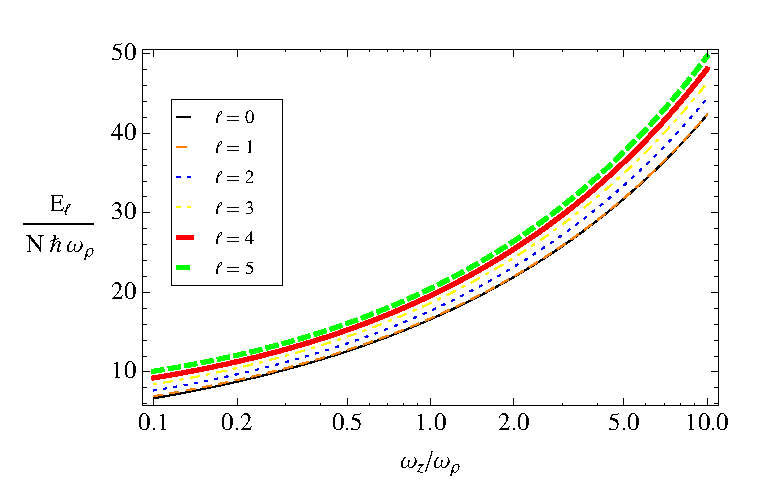
\includegraphics[scale=0.65]{1-FreeExpansionMultiplyCV-fig4}

\caption{Energy plotted as function of the trap anisotropy by fixing interaction
parameter as 800.}


\end{figure}


\begin{figure}
\centering
\captionsetup{labelfont=bf}

\subfloat[$\lambda=0.1$]{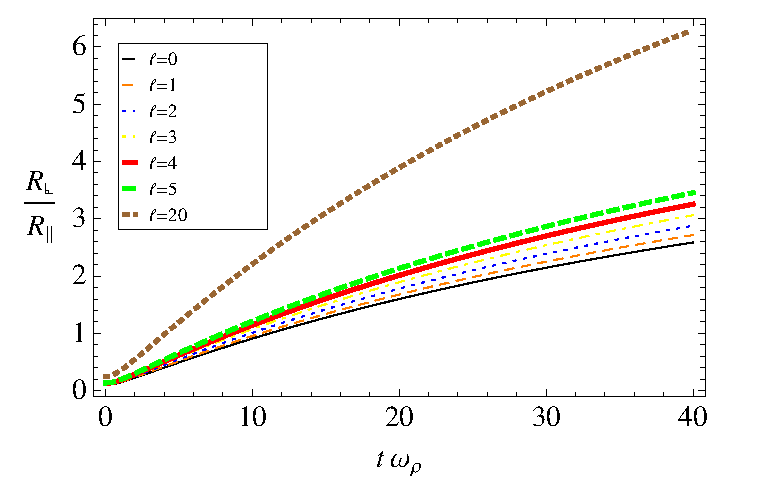
\includegraphics[scale=0.65]{1-FreeExpansionMultiplyCV-fig10}

}\subfloat[$\lambda=10$]{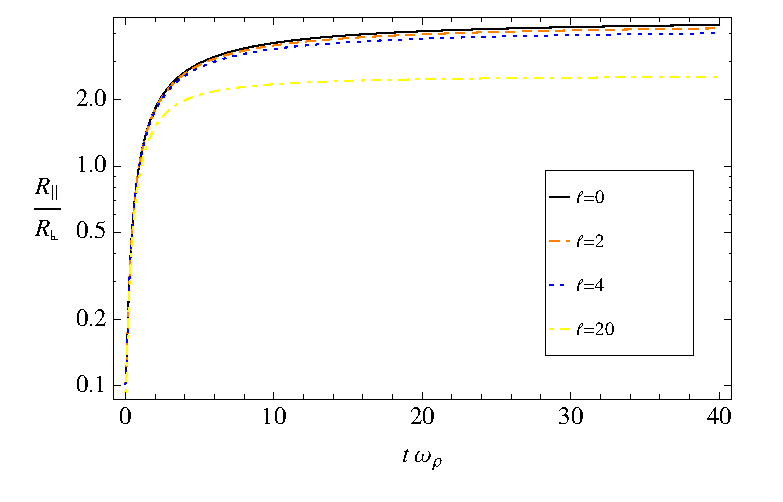
\includegraphics[scale=0.65]{1-FreeExpansionMultiplyCV-fig12}

}

\subfloat[$\lambda=1$]{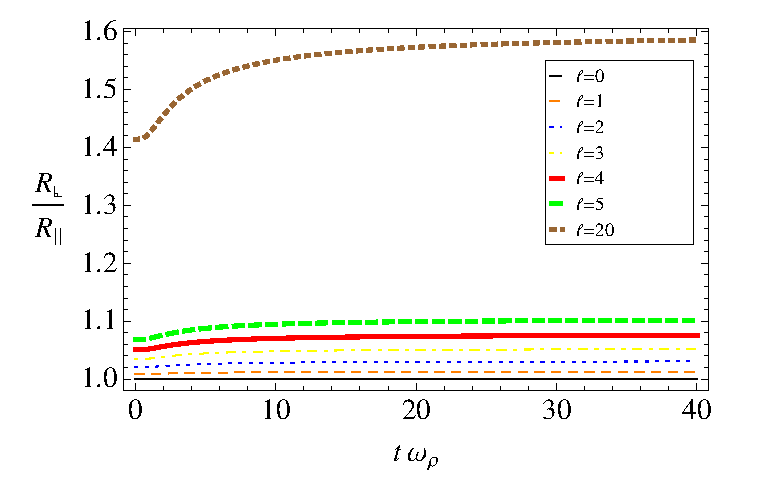
\includegraphics[scale=0.65]{1-FreeExpansionMultiplyCV-fig11}

}\subfloat[$\ell=1$]{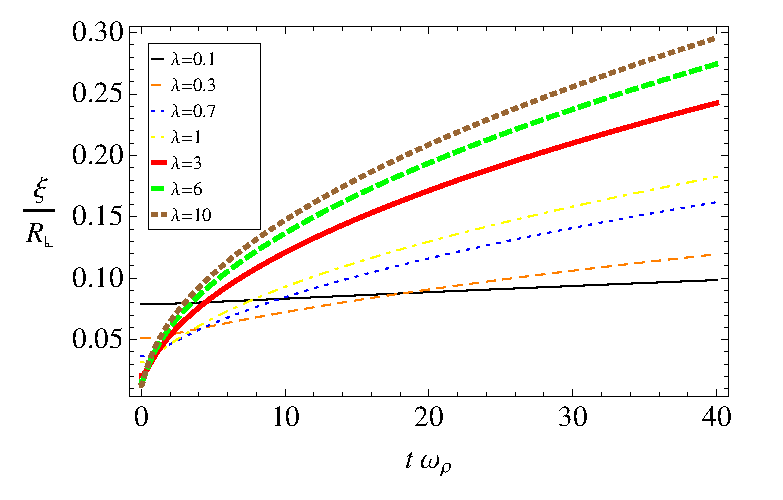
\includegraphics[scale=0.65]{1-FreeExpansionMultiplyCV-fig13}

}

\caption{Aspect ratio plotted while the free expansion for the respective trapped
shapes: (a) prolate shape, (b) oblate shape and (c) spherical shape.
They were calculated for $\gamma=800$. The plot of (d) represents
the ratio of vortex core by radial radius, while the free expansion,
for several kind of trap shapes.}
\end{figure}


\begin{figure}
\subfloat[$\lambda=0.1$]{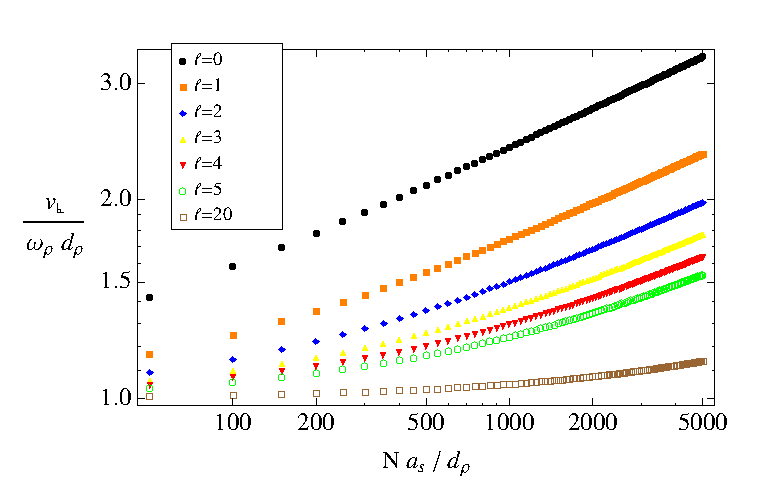
\includegraphics[scale=0.65]{1-FreeExpansionMultiplyCV-fig14}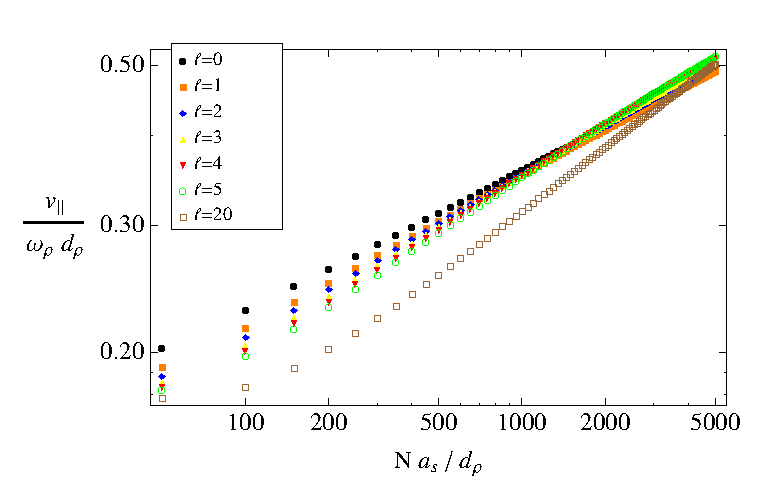
\includegraphics[scale=0.65]{1-FreeExpansionMultiplyCV-fig15}

}

\subfloat[$\lambda=10$]{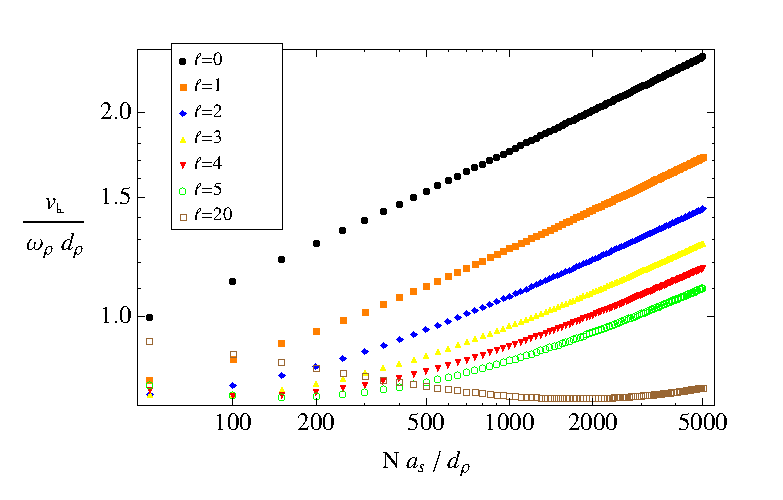
\includegraphics[scale=0.65]{1-FreeExpansionMultiplyCV-fig18}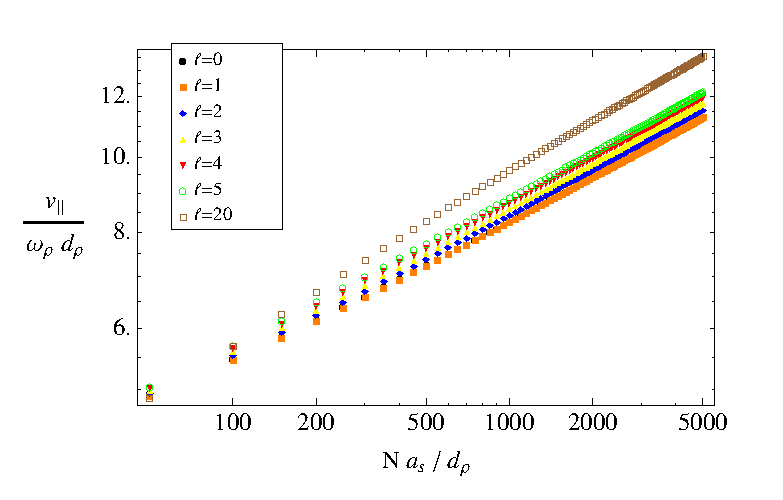
\includegraphics[scale=0.65]{1-FreeExpansionMultiplyCV-fig19}

}

\caption{The asymptotic behavior of expansion velocities with $\gamma$ for
the prolate and oblate shapes of initial potencial.}
\end{figure}


\begin{comment}
The method used gives us good results, where we have calculated the
initial conditions to the free expansion through \eqref{eq:3.2} by
Newton's method, and solved the equations\eqref{eq:4.2} by fourth-order
Runge-Kutta to flying time of the order of 30ms. Furthermore, all
of this graphic are to $\omega_{\rho}/2\pi=207Hz$ and $\gamma=800$,
because these values are the laboratory data from our experimental
group.

The approach \eqref{eq:2.6} proved to be usable for $\ell=1$, which
the case has the same energy when compared with the energy of $\ell=0$.
By checking $\xi^{(\ell)}$ for $\ell>1$, it was expected that $\xi^{(\ell)}$
was multiple of $\xi^{(1)}$ as it is known from literature\cite{pethick,aa},
i.e., $\xi^{(\ell)}=\ell\xi^{(1)}$. Although the result was $\xi^{(\ell)}<\ell\xi^{(1)}$,
in which case is justified by we may be observed the energy of a condensate
with fundamental vortex is the same of a condensate without vortex.
Thus, the vortex core is of the order of the healing length (condensate
without vortex) in the limit of Thomas-Fermi regime (Figure 1). Therefore,
the ratio $\xi/R_{\bot}$ while expansion just could be done for $\ell=1$
(Figure 4 (d)) such that agree qualitatively with numerical results
by F. Dalforo and M. Modugno\cite{michele}, and becomes better when
$\gamma\gg20$ as shown in the Figure 1. This results could be better
if we add the core size parameter in the trial function which greatly
complicates the equations.

In the expansion (Figure 4), we compared the time to aspect ratio
inversion for $\ell=0$ between this method and the data from experiments
($\omega_{\rho}=2\pi207Hz$, $\lambda\thickapprox0.1$ and $\gamma\thickapprox800$),
which resulted as a great crosscheck that is around 8ms.

Hence, as results, the vortex adds more kinetic energy and decrease
the interaction energy, which makes that condensate expand faster
in the orthogonal direction at the vortex's orientation. Furthermore,
it expands faster and faster to vortices with larger charge. Thus,
the inversion of the aspect ratio is faster when the trap shape is
prolate, and it slower when the condensate started the free expansion
from a oblate trap - as it has more charge on the vortex. Which these
can be explain by we are keeping $\omega_{\rho}$ fixed and varing
$\omega_{z}$. As known, the most confined direction of the condensate
expands faster, such that: to the spherical shape ($\lambda=1$),
the expansion is equal in both direction unless $\ell>0$. Consequently,
the vortex adds expansion's speed, however, it is not enough to cause
reversal in aspect ratio. Once the condensate containing the vortex
is slightly flatted at the poles.

The factor which have more influence in the aspect ratio inversion
is the kinetic potencial, this one has its importance at short times.
Thus its explan the faster aspect ratio inversion for $\ell>0$ at
$\lambda=0.1$, and for $\lambda=10$ the slower invesion of $\ell>0$
and $\ell=0$ is caused by the axial direction be most confined and
containg more quantum presure than other direction even though the
vortex contributes with centrifugal energy at this othogonal direction.

Thinking about the experimental problems in mensuring the time of
aspect ratio inversion at oblate shape of potencial ($\lambda>1$),
i.e., the range of these times are shortly and reach them assymptotical
expansion too fast. Thus we have calculated the assymptotical expansion
velocities for the both direction ($v_{\bot}$ and $v_{||}$), which
can be used to verify the Figure 1 (b) behavior by the Figure 2 (b).
\end{comment}


We solved eq. \ref{eq:4.2}, starting with the equilibrium configuration
inside the trap, to obtain the evolution of the parameters of the
condensate cloud during the free expansion. We used the frequency
($\omega_{\rho}=2\pi\times207Hz$) and expansion time (8ms) according
with our experiments with Rubidium 87 alkaline atoms.

To calculate the initial condition we use \eqref{eq:4.2} with the
acceleration equal to zero or minimize the energy function \eqref{eq:3.1}
in relation of the widths $r_{i}$ (reference of the appropriate equations
showed in the previous section).

The graphic 1 shows the initial energy of the system for a fixed interaction
parameter as function of the trap geometry (prolate\textendash{}isotropic-oblate
/ $\gamma$ (dimensionless) = 800 that correspond to real values in
the experiment $a_{s}=100a_{0}$. Number atoms in condensate = $10^{5}$)
for different circulations. The energy of the $\ell=1$ state differs
very little from the fundamental $\ell=0$ state, as it was expected
in the Thomas Fermi regime (TF). About the higher order circulation
states, this graphic shows an important physical effect that comes
from the vortex circulation. The latter brings nor only an extra kinetic
energy, but also affect the interaction energy since it spread the
condensate volume due to the centrifugal effect.

In the following we will analyze the evolution of the core during
the expansion. An important remark, however, is that our ansatz not
describe the correct behave of the vortex core, since it will be constrained
with the cloud dimensions. To improve such ansatz an additional parameter
should be used to characterize the core expansion independently. Since
we are in the TF regime, we used the relation between the vortex core
and condensate central density to describe such evolution (\eqref{eq:2.6}).
We represent the core equilibrium dimension together the approach
proposed, based on the density at $\rho=z=\ell=0$. It is clear that
the two sizes coincide to $\ell=1$ but for higher order of angular
momentum $\ell$ the ansatz start to fail, mostly when we are close
the oblate configuration, where the interaction energy is bigger \textendash{}
In this case our new characterization is even better \textendash{}
TF approach .

In the expansion (Figure 2), we compared the time to the aspect ratio
inversion for different circulations, starting with each type of magnetic
trap configuration.

The influences of the higher circulation are diferent for each intial
geometry of the condensate. For a spherical trap the dimensions of
the cloud is changed according with number of circulation, being that
in absence of vortex the condensate\textasciiacute{}s format is really
spherical in the other hand the vortex turns the aspect ratio greater
than 1, because this one reduces the axial radius and grows the radial
radius. In the prolate condensate, the circulation has an effect of
decreasing the time for aspect ratio invertion which can be interpreted
as the presence of the vortex has a significant addiction in the velocity
field on the perpendicular direction (Figure 2.a). It is just significant
when the perpendicular direction at vortex is the most confined. Thus
in the oposite case, when the intial geometry is oblate, the circulation
increases the time for aspect ratio invertion caused by fact the axial
radius smaller and smaller in the absence of centred atoms in the
cloud (Figure 2.b); even though the invertion time was lower in oblate
than prolate geometry.

Using the value for the core $\xi$ and the solution for the evolution
of the extension of the cloud given by eq. \ref{eq:4.2}, we analyze
how the vortex expand in relation to the cloud size. This analyze
is particularly important since it contributes to improve the information
that we extract from the absorption image technique made in time of
flight; for example, in the classification and quantification of the
number of vortex in the expanded cloud. The graphic of Figure 2.d
 shows the evolution of such ration in time for a cloud with unitary
circulation and starting with different trap anisotropy. The curves
can be explained basing on the variation of the central density due
to the trap configuration. For instance, the initial core size diminished
with the increase of $\lambda$ since the central density increases.
Otherwise the variation of the velocity of expansion in the axial
direction has direct consequence in the dilution of the density in
the vortex position, dictating its rate of expansion .

Comparing the graphs of the aspect ratios we notice a big difference
in the inversion time between Figure 2.a and Figure 2.b. Thus, we
think of a way to make a measurement for the prolate case which we
can distinguish each condensate, ie, to recognize and differentiate
the circulation of the vortex core condensate. The Figure 3 presents
the asymptotic velocity for both initial geometry (prolate and oblate)
as a function of the parameter of interaction, with these graphics
we hoped to find a critical phenomenon which, obviously, doesn't exist
at this framework. 





\pagebreak{}

\bibliographystyle{apsrev}
\bibliography{refdoc}

\end{document}
